% Created by tikzDevice version 0.12.6 on 2023-12-15 11:06:20
% !TEX encoding = UTF-8 Unicode
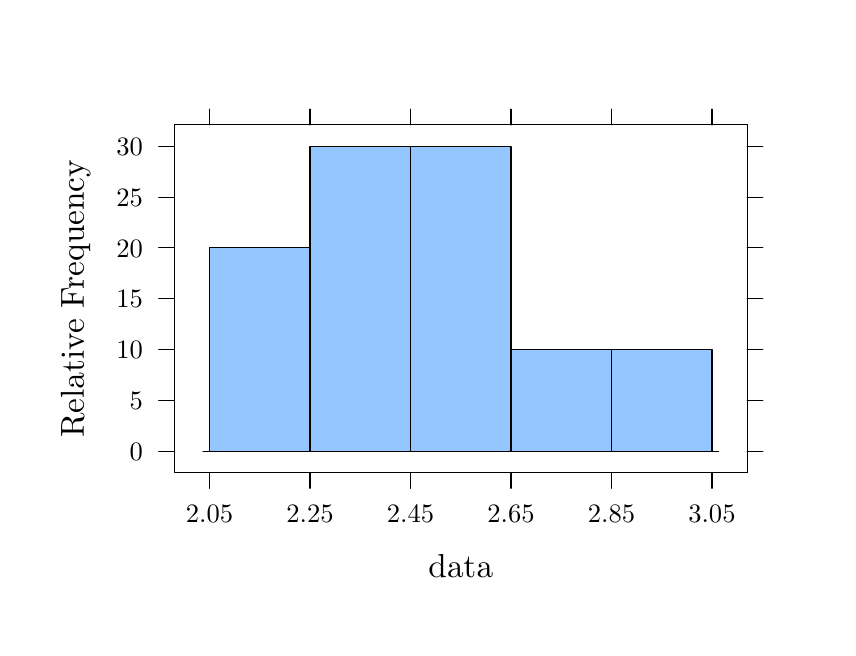
\begin{tikzpicture}[x=1pt,y=1pt]
\definecolor{fillColor}{RGB}{255,255,255}
\path[use as bounding box,fill=fillColor,fill opacity=0.00] (0,0) rectangle (289.08,216.81);
\begin{scope}
\path[clip] (  0.00,  0.00) rectangle (289.08,216.81);

\path[] (  0.00,  0.00) rectangle (289.08,216.81);
\definecolor{drawColor}{RGB}{0,0,0}

\node[text=drawColor,anchor=base,inner sep=0pt, outer sep=0pt, scale=  1.20] at (156.48, 18.07) {data};
\end{scope}
\begin{scope}
\path[clip] (  0.00,  0.00) rectangle (289.08,216.81);
\definecolor{drawColor}{RGB}{0,0,0}

\node[text=drawColor,rotate= 90.00,anchor=base,inner sep=0pt, outer sep=0pt, scale=  1.20] at ( 20.31,118.85) {Relative Frequency};
\end{scope}
\begin{scope}
\path[clip] (  0.00,  0.00) rectangle (289.08,216.81);
\definecolor{drawColor}{RGB}{0,0,0}

\path[draw=drawColor,line width= 0.4pt,line join=round,line cap=round] ( 65.71,181.67) -- ( 65.71,187.36);

\path[draw=drawColor,line width= 0.4pt,line join=round,line cap=round] (102.02,181.67) -- (102.02,187.36);

\path[draw=drawColor,line width= 0.4pt,line join=round,line cap=round] (138.33,181.67) -- (138.33,187.36);

\path[draw=drawColor,line width= 0.4pt,line join=round,line cap=round] (174.64,181.67) -- (174.64,187.36);

\path[draw=drawColor,line width= 0.4pt,line join=round,line cap=round] (210.95,181.67) -- (210.95,187.36);

\path[draw=drawColor,line width= 0.4pt,line join=round,line cap=round] (247.26,181.67) -- (247.26,187.36);
\end{scope}
\begin{scope}
\path[clip] (  0.00,  0.00) rectangle (289.08,216.81);
\definecolor{drawColor}{RGB}{0,0,0}

\path[draw=drawColor,line width= 0.4pt,line join=round,line cap=round] ( 53.00, 63.75) -- ( 47.31, 63.75);

\path[draw=drawColor,line width= 0.4pt,line join=round,line cap=round] ( 53.00, 82.12) -- ( 47.31, 82.12);

\path[draw=drawColor,line width= 0.4pt,line join=round,line cap=round] ( 53.00,100.49) -- ( 47.31,100.49);

\path[draw=drawColor,line width= 0.4pt,line join=round,line cap=round] ( 53.00,118.85) -- ( 47.31,118.85);

\path[draw=drawColor,line width= 0.4pt,line join=round,line cap=round] ( 53.00,137.22) -- ( 47.31,137.22);

\path[draw=drawColor,line width= 0.4pt,line join=round,line cap=round] ( 53.00,155.59) -- ( 47.31,155.59);

\path[draw=drawColor,line width= 0.4pt,line join=round,line cap=round] ( 53.00,173.96) -- ( 47.31,173.96);

\node[text=drawColor,anchor=base east,inner sep=0pt, outer sep=0pt, scale=  0.96] at ( 41.62, 60.45) {0};

\node[text=drawColor,anchor=base east,inner sep=0pt, outer sep=0pt, scale=  0.96] at ( 41.62, 78.81) {5};

\node[text=drawColor,anchor=base east,inner sep=0pt, outer sep=0pt, scale=  0.96] at ( 41.62, 97.18) {10};

\node[text=drawColor,anchor=base east,inner sep=0pt, outer sep=0pt, scale=  0.96] at ( 41.62,115.55) {15};

\node[text=drawColor,anchor=base east,inner sep=0pt, outer sep=0pt, scale=  0.96] at ( 41.62,133.92) {20};

\node[text=drawColor,anchor=base east,inner sep=0pt, outer sep=0pt, scale=  0.96] at ( 41.62,152.28) {25};

\node[text=drawColor,anchor=base east,inner sep=0pt, outer sep=0pt, scale=  0.96] at ( 41.62,170.65) {30};
\end{scope}
\begin{scope}
\path[clip] (  0.00,  0.00) rectangle (289.08,216.81);
\definecolor{drawColor}{RGB}{0,0,0}

\path[draw=drawColor,line width= 0.4pt,line join=round,line cap=round] ( 65.71, 56.04) -- ( 65.71, 50.35);

\path[draw=drawColor,line width= 0.4pt,line join=round,line cap=round] (102.02, 56.04) -- (102.02, 50.35);

\path[draw=drawColor,line width= 0.4pt,line join=round,line cap=round] (138.33, 56.04) -- (138.33, 50.35);

\path[draw=drawColor,line width= 0.4pt,line join=round,line cap=round] (174.64, 56.04) -- (174.64, 50.35);

\path[draw=drawColor,line width= 0.4pt,line join=round,line cap=round] (210.95, 56.04) -- (210.95, 50.35);

\path[draw=drawColor,line width= 0.4pt,line join=round,line cap=round] (247.26, 56.04) -- (247.26, 50.35);

\node[text=drawColor,anchor=base,inner sep=0pt, outer sep=0pt, scale=  0.96] at ( 65.71, 38.05) {2.05};

\node[text=drawColor,anchor=base,inner sep=0pt, outer sep=0pt, scale=  0.96] at (102.02, 38.05) {2.25};

\node[text=drawColor,anchor=base,inner sep=0pt, outer sep=0pt, scale=  0.96] at (138.33, 38.05) {2.45};

\node[text=drawColor,anchor=base,inner sep=0pt, outer sep=0pt, scale=  0.96] at (174.64, 38.05) {2.65};

\node[text=drawColor,anchor=base,inner sep=0pt, outer sep=0pt, scale=  0.96] at (210.95, 38.05) {2.85};

\node[text=drawColor,anchor=base,inner sep=0pt, outer sep=0pt, scale=  0.96] at (247.26, 38.05) {3.05};

\path[draw=drawColor,line width= 0.4pt,line join=round,line cap=round] (259.96, 63.75) -- (265.65, 63.75);

\path[draw=drawColor,line width= 0.4pt,line join=round,line cap=round] (259.96, 82.12) -- (265.65, 82.12);

\path[draw=drawColor,line width= 0.4pt,line join=round,line cap=round] (259.96,100.49) -- (265.65,100.49);

\path[draw=drawColor,line width= 0.4pt,line join=round,line cap=round] (259.96,118.85) -- (265.65,118.85);

\path[draw=drawColor,line width= 0.4pt,line join=round,line cap=round] (259.96,137.22) -- (265.65,137.22);

\path[draw=drawColor,line width= 0.4pt,line join=round,line cap=round] (259.96,155.59) -- (265.65,155.59);

\path[draw=drawColor,line width= 0.4pt,line join=round,line cap=round] (259.96,173.96) -- (265.65,173.96);
\end{scope}
\begin{scope}
\path[clip] ( 53.00, 56.04) rectangle (259.96,181.67);
\definecolor{drawColor}{RGB}{0,0,0}

\path[draw=drawColor,line width= 0.4pt,line join=round,line cap=round] ( 63.35, 63.75) --
	(249.62, 63.75);
\definecolor{fillColor}{RGB}{148,198,255}

\path[draw=drawColor,line width= 0.4pt,line join=round,line cap=round,fill=fillColor] ( 65.71, 63.75) rectangle (102.02,137.22);

\path[draw=drawColor,line width= 0.4pt,line join=round,line cap=round,fill=fillColor] (102.02, 63.75) rectangle (138.33,173.96);

\path[draw=drawColor,line width= 0.4pt,line join=round,line cap=round,fill=fillColor] (138.33, 63.75) rectangle (174.64,173.96);

\path[draw=drawColor,line width= 0.4pt,line join=round,line cap=round,fill=fillColor] (174.64, 63.75) rectangle (210.95,100.49);

\path[draw=drawColor,line width= 0.4pt,line join=round,line cap=round,fill=fillColor] (210.95, 63.75) rectangle (247.26,100.49);
\end{scope}
\begin{scope}
\path[clip] (  0.00,  0.00) rectangle (289.08,216.81);
\definecolor{drawColor}{RGB}{0,0,0}

\path[draw=drawColor,line width= 0.4pt,line join=round,line cap=round] ( 53.00, 56.04) rectangle (259.96,181.67);
\end{scope}
\end{tikzpicture}
